\documentclass[class=article, crop=false]{standalone}
\usepackage[subpreambles=true]{standalone}
\usepackage{import}
\usepackage[T1]{fontenc}
\usepackage[utf8]{inputenc}
\usepackage[english, danish]{babel}
\usepackage{graphicx,wrapfig,lipsum}

\begin{document}
    I denne afsnit beskrives sekvensdiagrammer over de mest essentielle operationer i systemet i vores øjne.
    \paragraph{LandedOn\\}
Sekvensdiagrammet på Figur~\ref{fig:SD_landed_on} illustrerer de operationer, der foregår, når en spiller tager sin tur og lander på et felt. Der blev benyttet Visitor pattern til landedOn metoden til at optimere forståelsen af koden. Visitor pattern kan der læses videre på sektion~\ref{sec:visitor}
    \begin{figure}[H]

\hbox{\hspace{-0cm}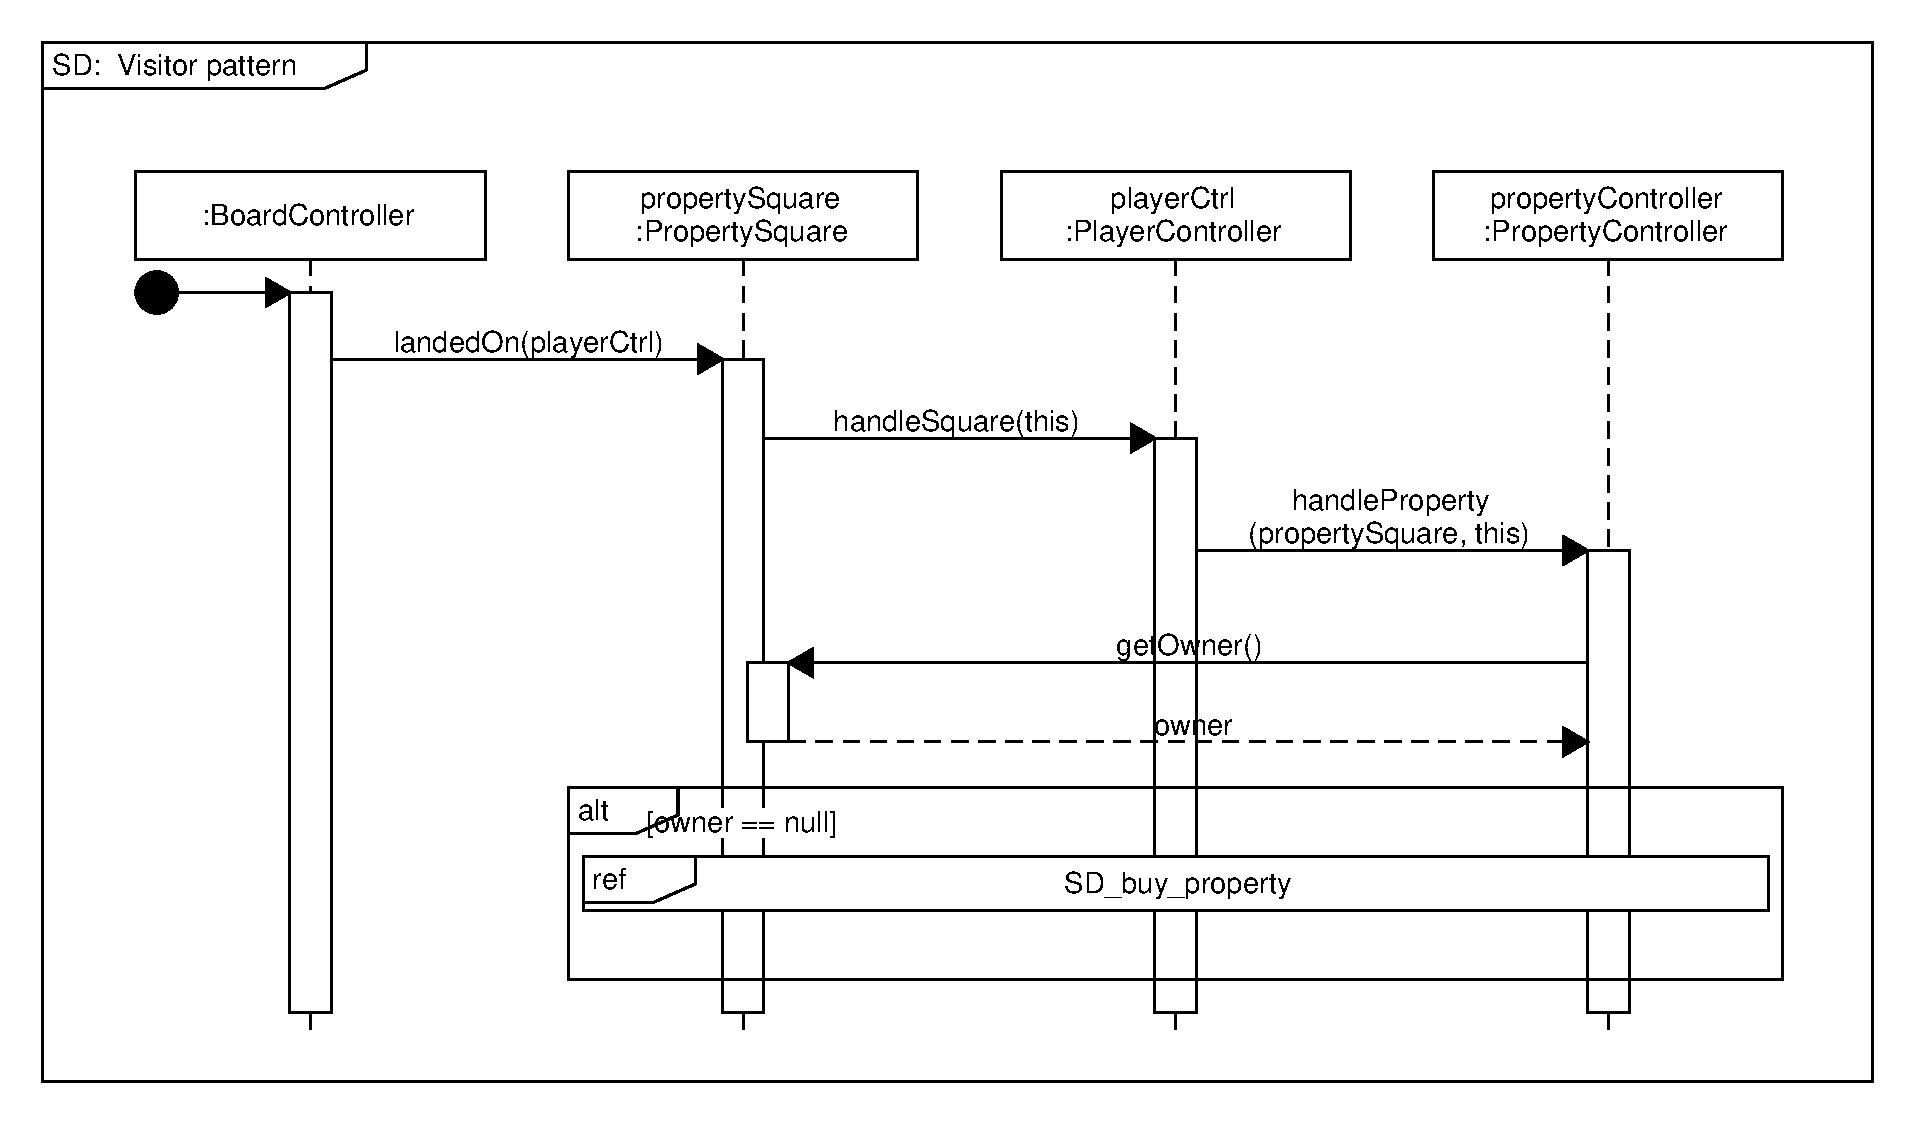
\includegraphics[scale=0.7]{diagrams/SD_landed_on.pdf}}

        \caption{Sekvensdiagrammet over landedOn metoden}\label{fig:SD_landed_on}
    \end{figure}
    \newpage
    \paragraph{BuyProperty\\}
    Sekvensdiagrammet på Figur~\ref{fig:SD_buy_property} illustrerer de operationer, der foregår, når en spiller købe en grund.
    \begin{figure}[H]

\hbox{\hspace{-2cm}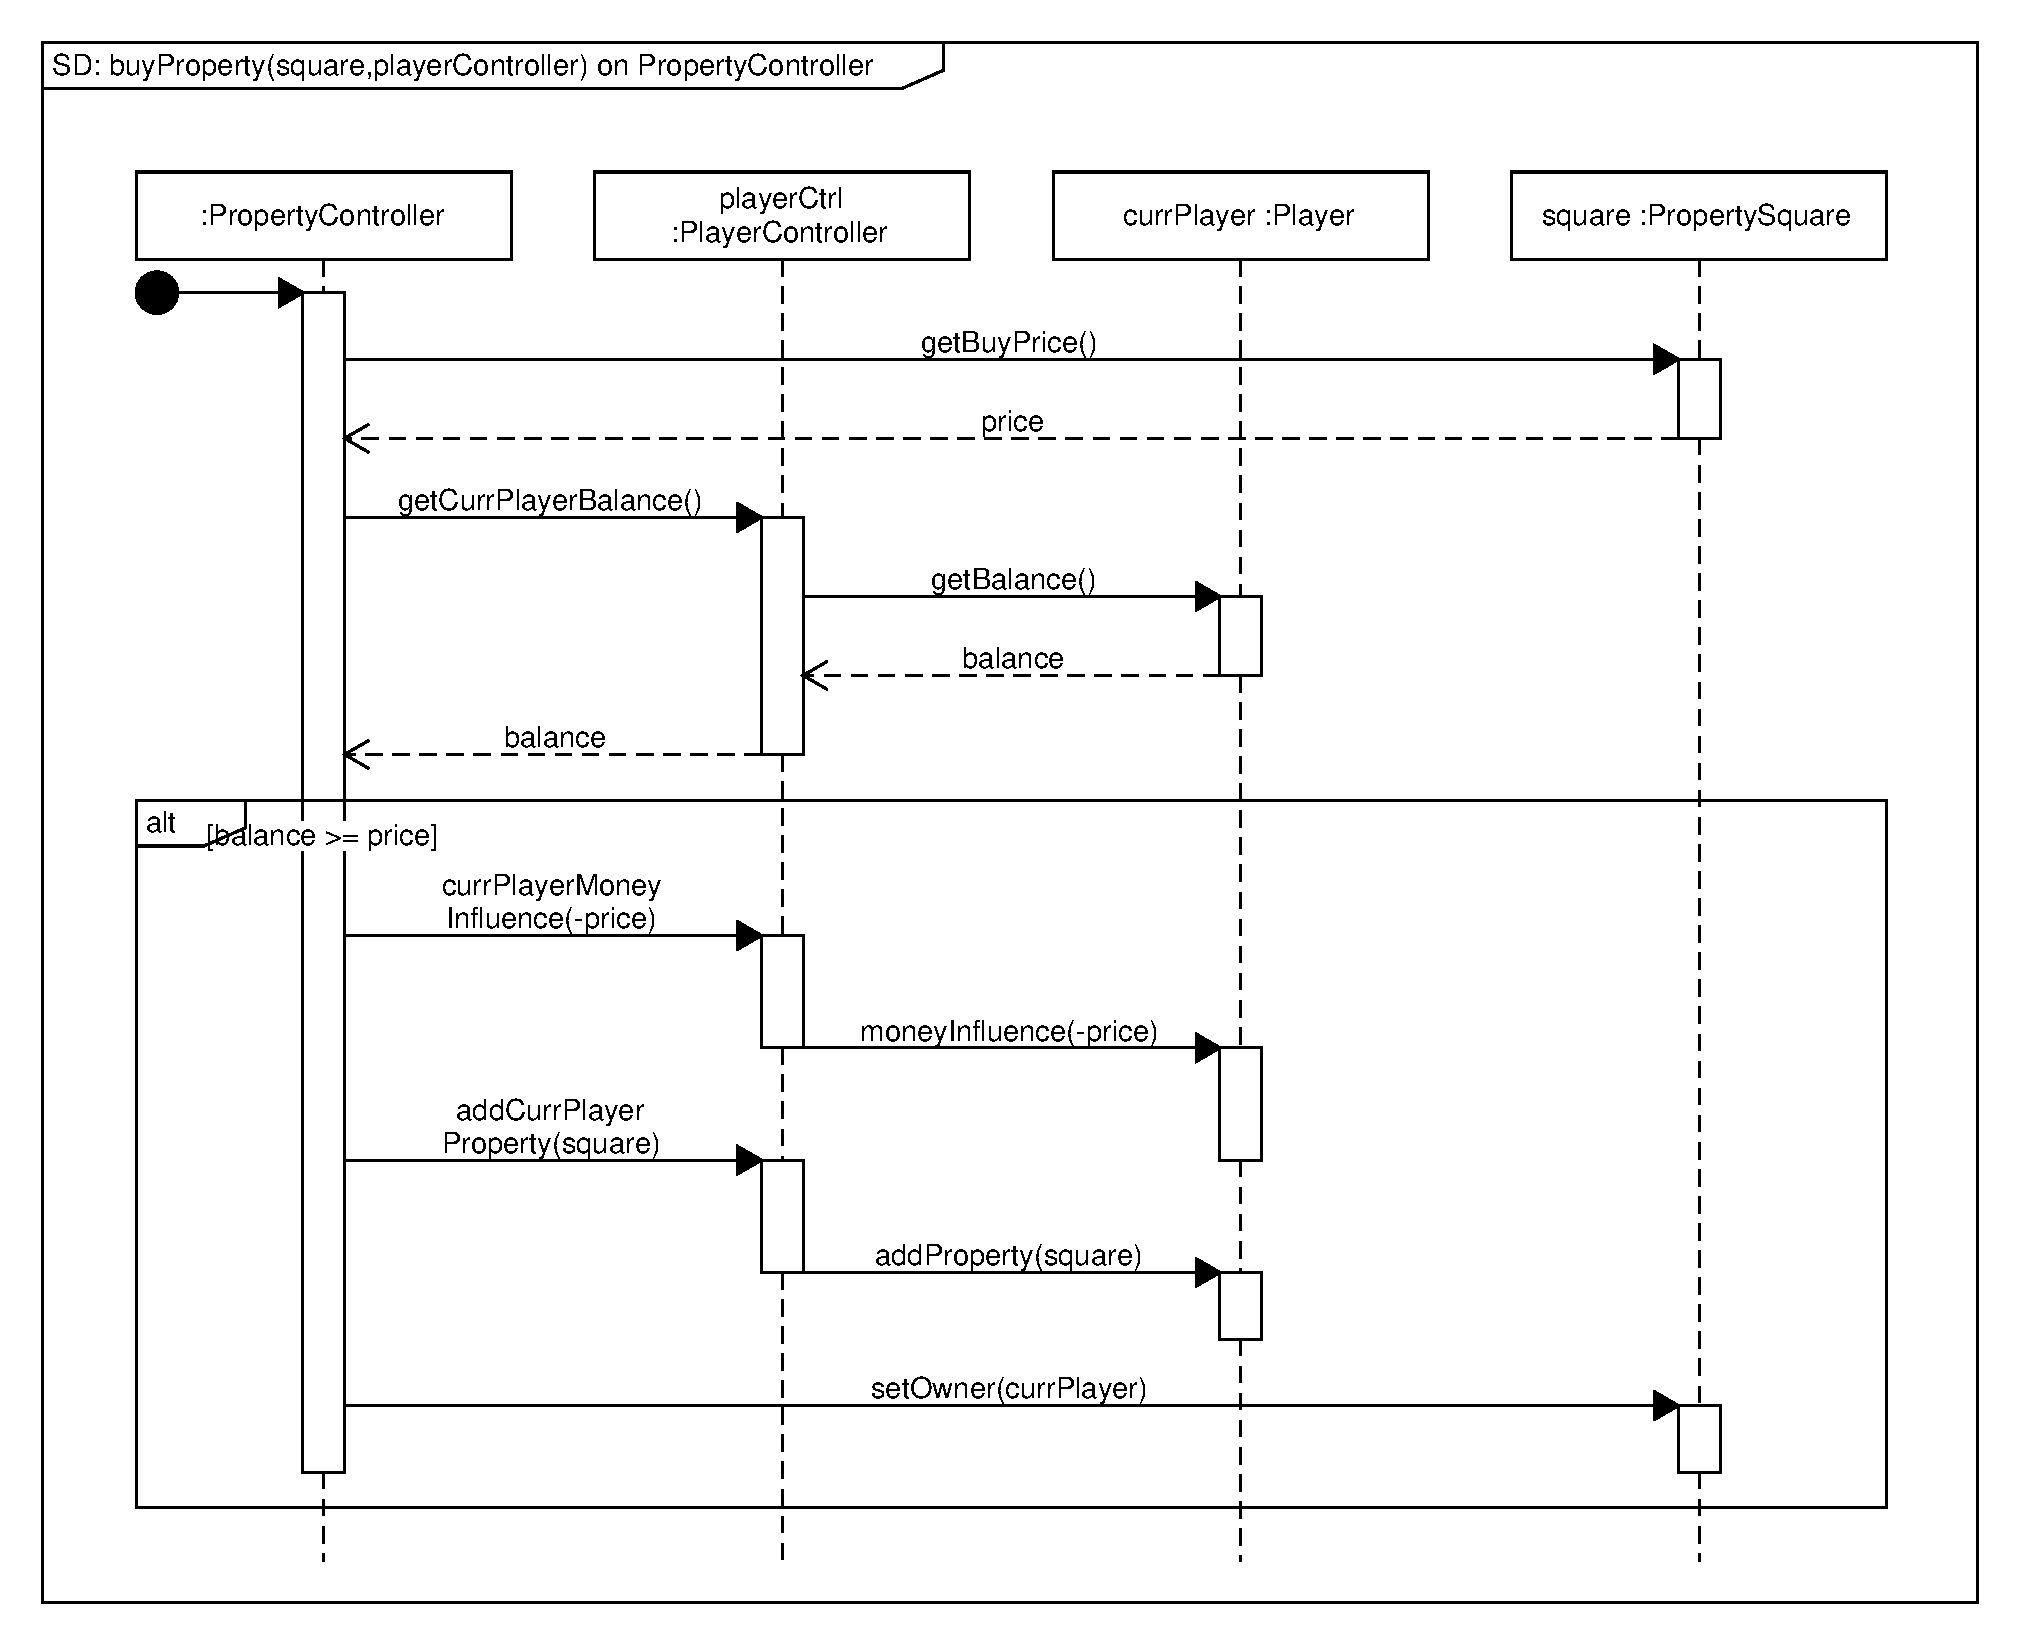
\includegraphics[scale=0.6]{diagrams/SD_buy_property.pdf}}

        \caption{Sekvensdiagrammet over buyProperty metoden}\label{fig:SD_buy_property}
    \end{figure}
    \newpage
    \paragraph{PayRent\\}
    Sekvensdiagrammet på Figur~\ref{fig:SD_pay_rent} illustrerer de operationer, der foregår, når en spiller betaler leje.
    \begin{figure}[H]

\hbox{\hspace{-2.7cm}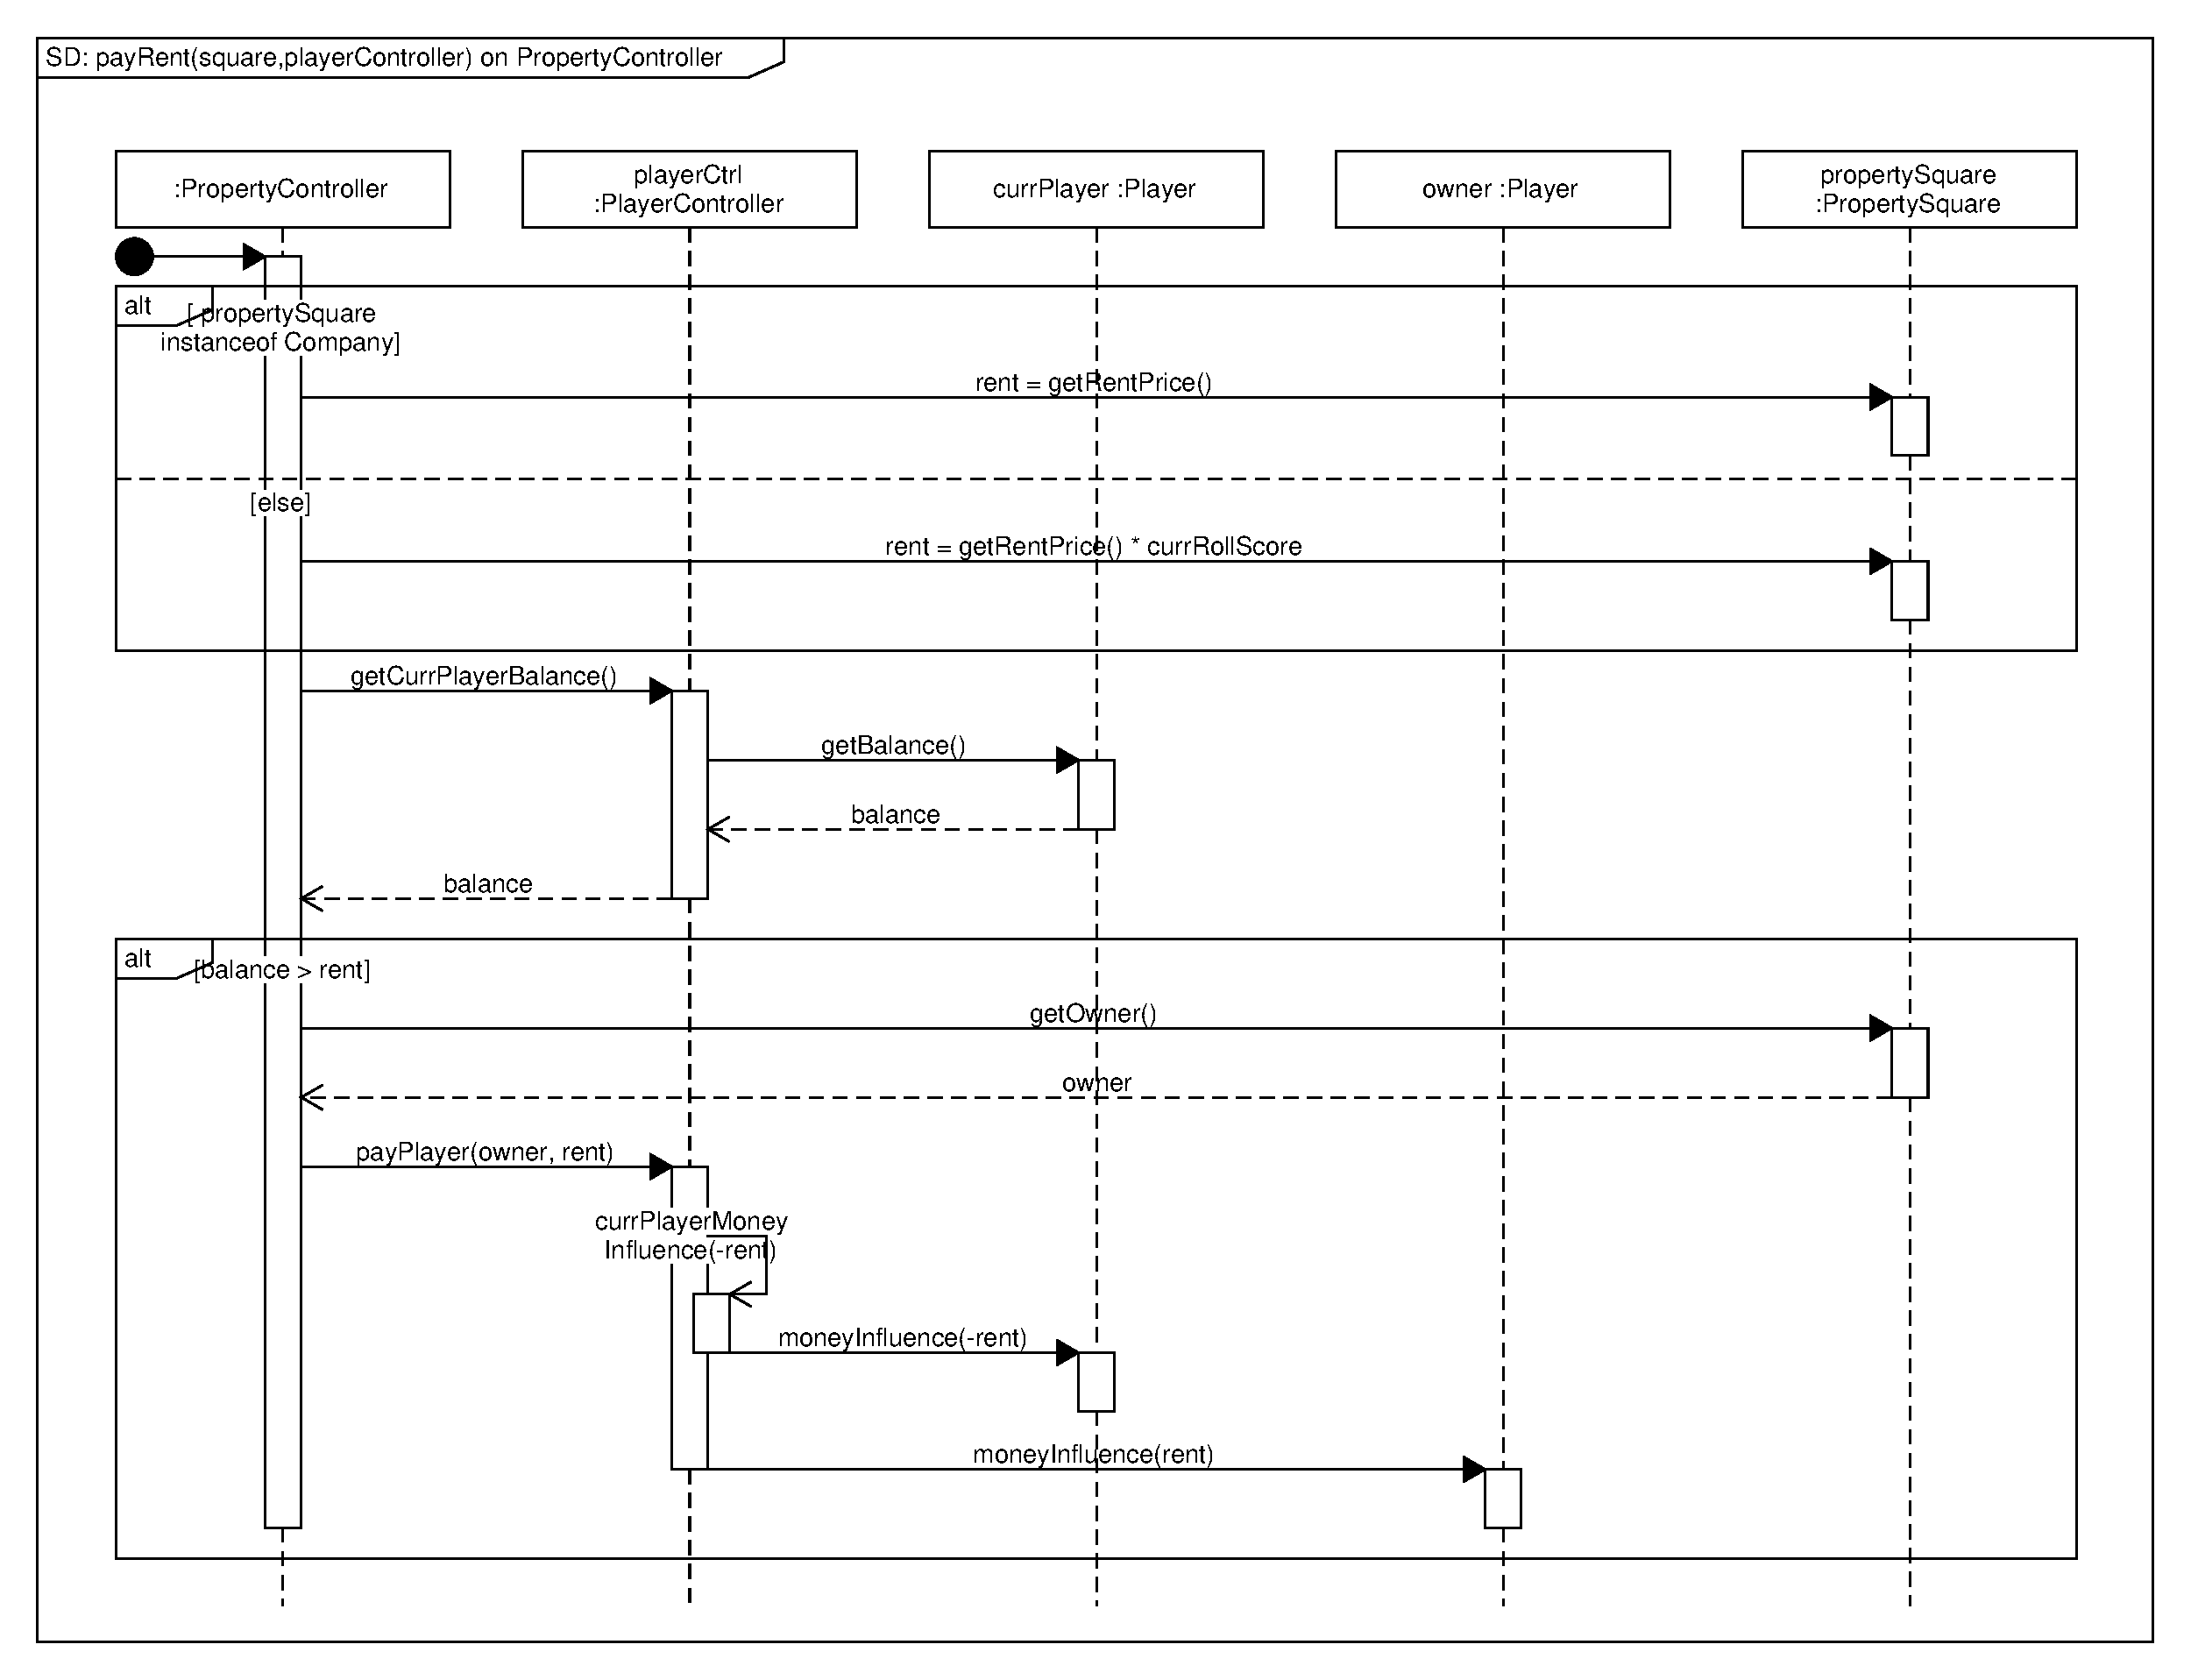
\includegraphics[scale=0.54]{diagrams/SD_pay_rent.pdf}}

        \caption{Sekvensdiagrammet over payRent metoden}\label{fig:SD_pay_rent}
    \end{figure}
    \newpage
\end{document}